\documentclass[UTF8,a4paper,12pt]{ctexart}

\usepackage{geometry}
\usepackage{graphicx}
\usepackage{booktabs}
\usepackage{longtable}
\usepackage{array}
\usepackage{amsmath}
\usepackage{float}
\usepackage{xcolor}
\usepackage{listings}
\usepackage{hyperref}
\usepackage{enumitem}
\usepackage{fancyhdr}
\usepackage{caption}
\usepackage{subcaption}
\usepackage{titlesec}

\geometry{left=2.6cm,right=2.6cm,top=2.7cm,bottom=2.7cm}
\graphicspath{{assets/}}
\hypersetup{
  colorlinks=true,
  linkcolor=black,
  urlcolor=blue!55!black,
  citecolor=black
}
\setlength{\parindent}{2em}
\setlength{\parskip}{0.25em}
\setlength{\headheight}{15pt}
\emergencystretch=2em
\setlist{nosep}
\captionsetup{font=small,labelsep=quad}

\definecolor{codegreen}{RGB}{27,112,78}
\definecolor{codegray}{RGB}{100,110,105}
\definecolor{codebg}{RGB}{246,249,247}
\lstset{
  basicstyle=\ttfamily\small,
  backgroundcolor=\color{codebg},
  frame=single,
  rulecolor=\color{black!12},
  breaklines=true,
  columns=fullflexible,
  keywordstyle=\color{codegreen},
  commentstyle=\color{codegray},
  showstringspaces=false
}

\pagestyle{fancy}
\fancyhf{}
\fancyhead[L]{数字图像处理实验报告}
\fancyhead[R]{基于 YOLOv5 的有害垃圾检测系统}
\fancyfoot[C]{\thepage}

\titleformat{\section}{\Large\bfseries}{\thesection}{1em}{}
\titleformat{\subsection}{\large\bfseries}{\thesubsection}{1em}{}

\begin{document}

\begin{titlepage}
  \centering
  \vspace*{2.2cm}
  {\heiti\zihao{1} 数字图像处理实验报告\par}
  \vspace{1.1cm}
  {\heiti\zihao{2} 基于 YOLOv5 的有害垃圾智能检测系统\par}
  \vspace{0.5cm}
  {\Large 面向混合垃圾场景的有害垃圾快速筛查\par}
  \vfill
  \renewcommand{\arraystretch}{1.8}
  \begin{tabular}{>{\bfseries}p{3.5cm}p{7cm}}
    项目成员： & 刘晋嶂、邓荣基、袁致朗 \\
    模型训练： & 刘晋嶂 \\
    图像处理： & 邓荣基 \\
    技术调研与报告： & 袁致朗 \\
    完成日期： & 2026 年 6 月 \\
  \end{tabular}
  \vfill
  {\large 基于数字图像处理与深度学习目标检测技术\par}
\end{titlepage}

\begin{abstract}
在生活垃圾收集、转运和分拣过程中，干电池、过期药品、药膏及其他具有毒性、腐蚀性或潜在环境危害的物品，可能被混入大量普通垃圾。若这些有害垃圾未在前端及时识别并分离，它们可能进入压缩、破碎、焚烧、填埋或资源化利用等后续环节，造成有害物质泄漏、设备污染和二次环境风险。与此同时，环卫工人面对的通常不是背景干净、摆放规则的单件垃圾，而是数量庞大、相互遮挡且外观复杂的混合垃圾，单纯依靠人工逐件检查效率低、劳动强度高，并可能增加直接接触风险。

本项目围绕上述现实问题，设计并实现了一套基于 YOLOv5s 的垃圾目标检测系统。系统首先使用数字图像处理流水线对上传图像进行尺寸归一化、Gaussian Blur 去噪、CLAHE 局部对比度增强及 Unsharp Masking 锐化，再由 YOLOv5s 对图像中的垃圾进行分类与定位。当检测结果中出现干电池、过期药品、药膏、充电宝和化妆品瓶等有害垃圾时，Web 前端会进行醒目提示。实验采用开源且已完成目标框标注的垃圾图像数据集进行迁移学习，最终模型在验证集上获得 Precision 0.5476、Recall 0.5506、mAP@0.5 0.5612 和 mAP@0.5:0.95 0.3408。结果表明，本项目实现了从图像预处理、模型训练到前端部署的完整流程，并初步验证了利用视觉检测技术辅助环卫人员快速筛查有害垃圾的可行性。

\noindent\textbf{关键词：} 有害垃圾；目标检测；YOLOv5；图像预处理；垃圾分类；环境保护
\end{abstract}

\newpage
\tableofcontents
\newpage

\section{项目介绍}

\subsection{项目背景}

生活垃圾处理并不是单一的“投放后消失”过程，而是一条包含收集、运输、暂存、分拣、压缩、破碎、焚烧、填埋和资源化利用等环节的处理链条。若干电池、过期药品等有害垃圾在源头被混入普通垃圾，污染风险会沿着处理链向下游传递。例如，电池破损后可能释放电解液和重金属；药品包装或残留药物可能进入渗滤液；部分含化学物质的容器在压缩、破碎和焚烧过程中还可能带来额外风险。

在现实工作中，环卫工人需要从大量混合垃圾中发现这些目标。人工检查具有直观性，但存在三个明显限制：第一，垃圾数量大、更新速度快，逐件检查的时间成本高；第二，垃圾堆中目标常被遮挡、污染或压扁，容易漏检；第三，直接翻找可能使工作人员接触尖锐、腐蚀性或存在卫生风险的物品。因此，能够在图像中自动定位可疑有害垃圾的视觉系统，可以作为人工分拣前的一道辅助筛查工具。

\subsection{项目目标与现实价值}

本项目的核心目标不是取代环卫工人，而是为其提供一种快速、低接触的辅助判断方式。工作人员可以对垃圾堆或待分拣区域拍照，系统在短时间内给出垃圾类别、位置和置信度，并对有害垃圾进行重点提醒。其现实价值主要体现在以下方面：

\begin{enumerate}
  \item \textbf{提高筛查效率。} 系统能够同时检查图像中的多个目标，帮助工作人员优先关注疑似有害垃圾区域，减少盲目翻找。
  \item \textbf{降低职业接触风险。} 先通过图像完成初步筛查，可以减少工作人员直接接触未知垃圾的频率。
  \item \textbf{阻断污染向下游传播。} 尽早将有害垃圾从普通垃圾流中分离，有助于降低其进入压缩、破碎、焚烧和填埋环节后造成污染的可能性。
  \item \textbf{形成可扩展的技术基础。} 当前系统可部署为本地 Web 应用，未来可进一步接入固定摄像头、移动终端或垃圾分拣设备。
\end{enumerate}

\subsection{系统功能与技术路线}

系统采用“图像预处理---目标检测---风险判定---前端展示”的技术路线。用户上传图片后，系统首先增强图像质量，再使用 YOLOv5s 识别并定位垃圾。当检测类别属于预先定义的有害垃圾集合时，前端以红色警告框进行重点提醒。

\begin{figure}[H]
  \centering
  \fbox{\parbox{0.88\textwidth}{
    \centering
    上传垃圾图片
    $\longrightarrow$ Resize
    $\longrightarrow$ Gaussian Blur
    $\longrightarrow$ CLAHE
    $\longrightarrow$ Sharpen
    $\longrightarrow$ YOLOv5s
    $\longrightarrow$ 类别与位置输出
    $\longrightarrow$ 有害垃圾告警
  }}
  \caption{系统整体处理流程}
\end{figure}

\section{数据采集与处理的详细过程}

\subsection{早期数据采集尝试}

项目初期，团队尝试通过自行拍摄和使用生成式 AI 辅助生成图片的方式构建数据集。自行拍摄能够获得与实际场景接近的图像，但受时间、垃圾类别、拍摄条件和标注成本限制，短时间内能够获得的有效样本数量非常有限。AI 生成图片可以补充部分外观变化，但生成图像与真实垃圾堆在遮挡关系、污损程度、光照和背景复杂度方面仍存在差异，并且生成后仍需人工检查和标注。

在使用这一小规模数据进行早期训练后，模型表现较差。其根本原因在于目标检测模型不仅需要认识物体的典型外观，还需要学习不同尺度、角度、光照、遮挡和背景条件下的变化。少量且分布单一的图片容易导致模型过拟合：它可能记住训练图片，却无法稳定识别新的垃圾照片。

\subsection{采用开源标注数据集}

为解决样本数量与标注质量不足的问题，团队转而调研网络上的开源垃圾图片数据集。调研发现，已有数据集包含多种生活垃圾图像，并已提供目标框和类别标签，可按 YOLO 标准格式组织为 \texttt{images} 与 \texttt{labels} 目录，其中训练集和验证集分别放置在 \texttt{train} 与 \texttt{val} 子目录。

采用现有标注数据集具有明确的工程价值：一方面，大规模样本为模型学习真实外观差异提供基础；另一方面，已有标注可以显著减少重复劳动，使团队能够将更多精力投入图像处理、训练参数调整和应用部署。当前模型共包含 40 个垃圾类别，其中与有害垃圾筛查直接相关的类别包括 \texttt{DryBattery}、\texttt{ExpiredDrugs}、\texttt{Ointment}、\texttt{Powerbank} 和 \texttt{CosmeticBottles}。

\begin{figure}[H]
  \centering
  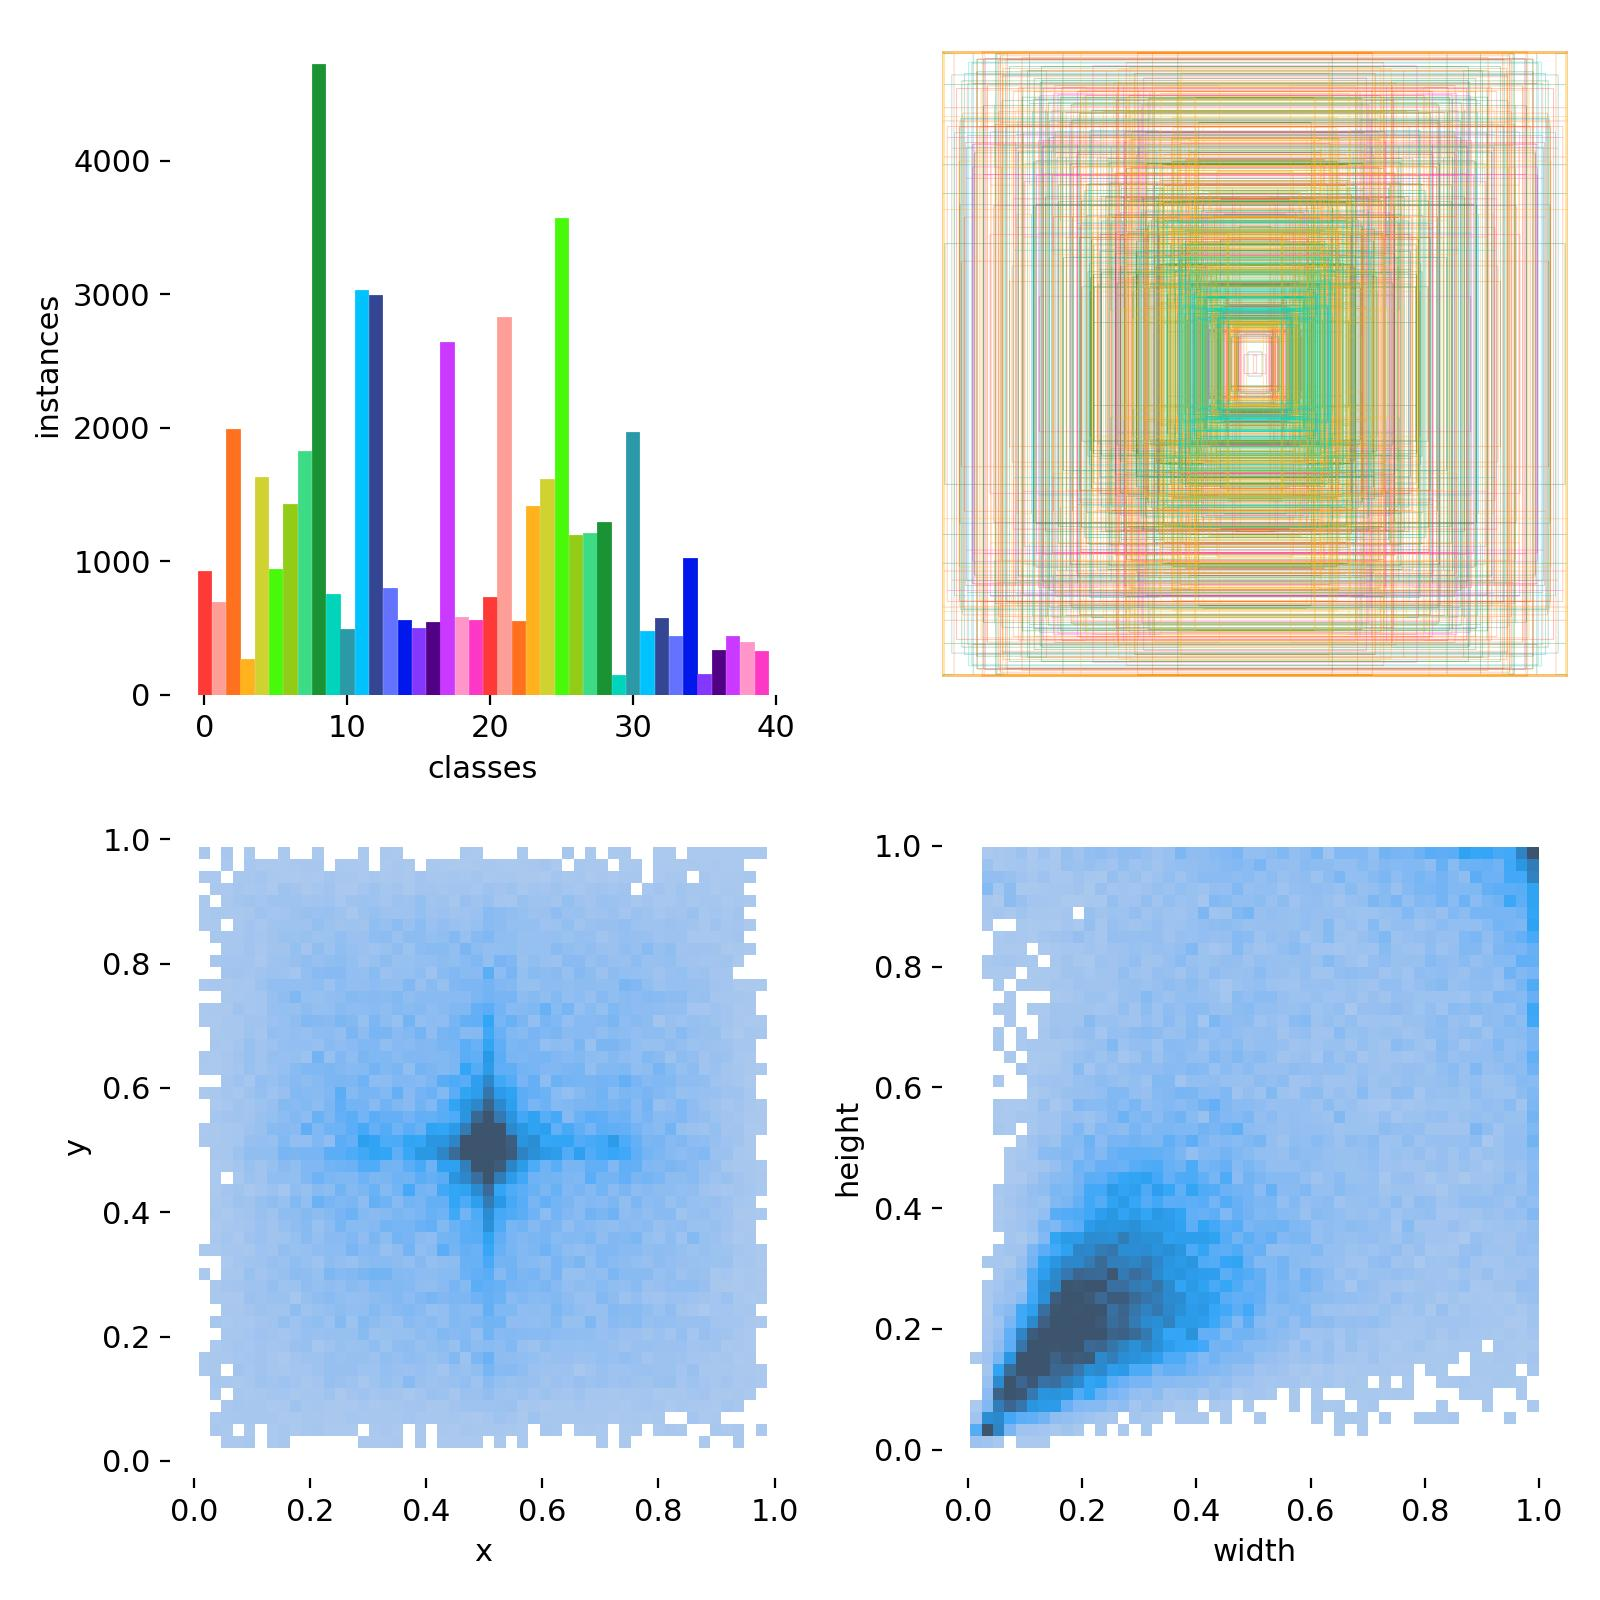
\includegraphics[width=0.82\textwidth]{labels.jpg}
  \caption{数据集目标框与类别分布可视化}
\end{figure}

\subsection{图像预处理流程}

为了改善拍摄图片中尺寸过大、局部对比度不足、噪声和边缘模糊等问题，项目在根目录的 \texttt{preprocess.py} 中实现了完整预处理流程，并将其接入 Web 检测 Pipeline。预处理不仅服务于模型输入，还对应真实使用场景中的具体问题。

\begin{longtable}{p{3.1cm}p{4.2cm}p{7.0cm}}
  \toprule
  处理组件 & 参数设置 & 现实作用与设计目的 \\
  \midrule
  \endhead
  Resize & 长边最大为 1280，保持宽高比，使用 \texttt{INTER\_AREA} & 控制高分辨率手机照片的计算量和内存占用，同时避免非等比例缩放造成垃圾外形失真。\\
  Gaussian Blur & $3\times3$ 高斯核 & 减弱拍摄噪声、压缩噪声和细碎纹理干扰，使模型更关注稳定的形状和区域特征。\\
  CLAHE & \texttt{clipLimit=2.0}，网格大小 $8\times8$，在 LAB 空间 L 通道处理 & 增强阴影、光照不均和局部低对比度区域，使垃圾堆中较暗或与背景接近的目标更容易被观察。\\
  Unsharp Masking & 模糊核 $5\times5$，强度 1.5 & 强化目标边缘与结构信息，帮助模型区分轮廓相近或边界模糊的垃圾目标。\\
  \bottomrule
\end{longtable}

\begin{figure}[H]
  \centering
  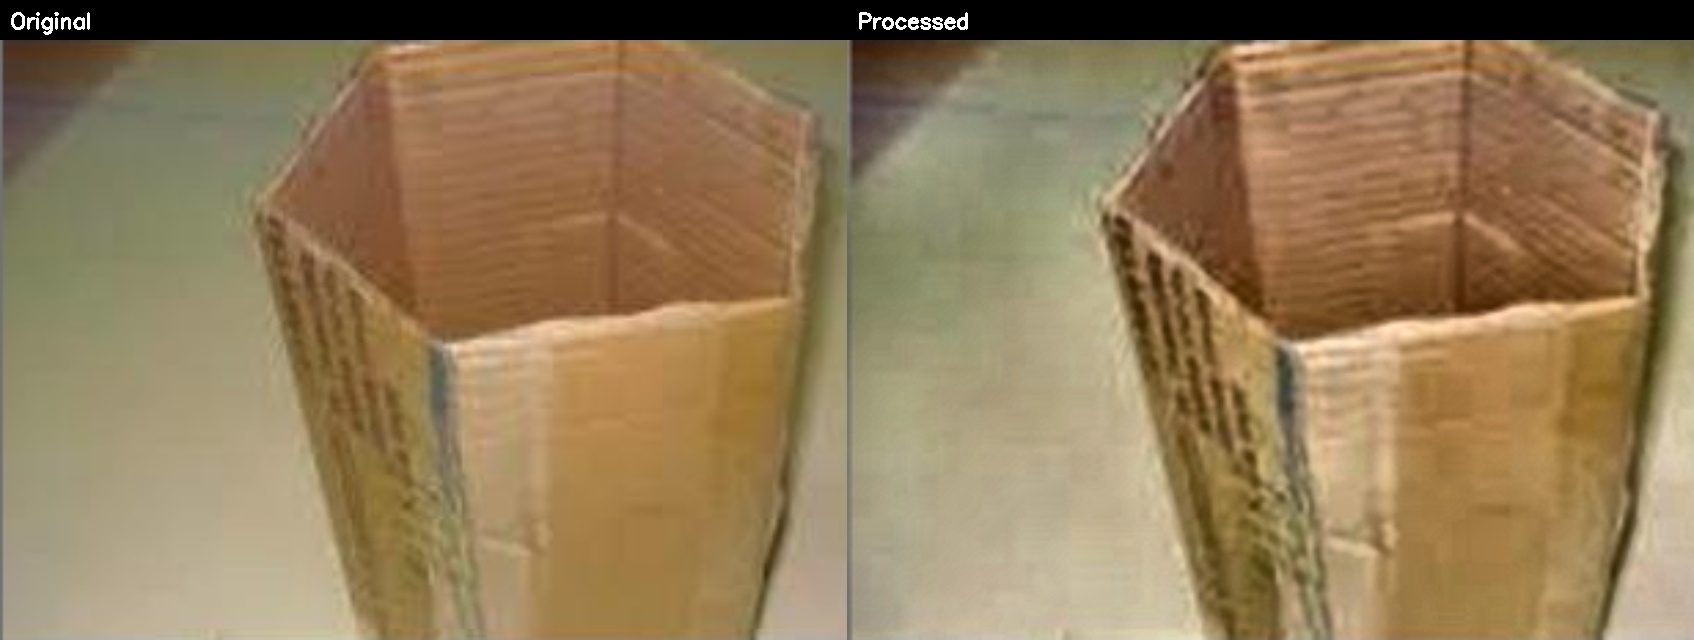
\includegraphics[width=\textwidth]{preprocess_comparison.jpg}
  \caption{图像预处理前后对比}
\end{figure}

核心处理代码如下：

\begin{lstlisting}[language=Python,caption={图像预处理核心流程}]
def preprocess(img):
    img = resize_image(img, max_size=1280)
    img = denoise_gaussian(img, kernel=3)
    img = enhance_clahe(img, clip_limit=2.0, tile_size=8)
    img = sharpen_unsharp(img, strength=1.5)
    return img
\end{lstlisting}

\subsection{数据划分与标注格式}

数据集使用训练集学习模型参数，使用验证集观察泛化性能并选择最佳权重。每张图片对应一个文本标签文件，每行记录类别编号及归一化后的目标框中心坐标、宽度和高度。该组织方式能够直接被 YOLOv5 的训练脚本读取。需要指出的是，验证集必须与训练集保持独立，否则验证指标会高估模型面对新图片时的能力。

\section{YOLOv5s 模型与训练参数}

\subsection{选择 YOLOv5s 的原因}

YOLO 系列将目标分类与位置回归整合到一次前向推理中，适合需要快速反馈的目标检测场景。YOLOv5s 属于较轻量的模型版本，在计算资源有限时能够兼顾检测速度与精度，也便于在普通电脑上完成推理和 Web 部署。因此，本实验使用 YOLOv5s 作为基线模型，并基于预训练权重进行迁移学习。

\subsection{YOLOv5s 训练参数设置}

本实验采用 YOLOv5s 作为目标检测模型，并基于预训练权重 \texttt{yolov5s.pt} 进行迁移学习。训练数据集采用 YOLO 标准格式进行组织，图像文件与标签文件分别存放在 \texttt{images} 和 \texttt{labels} 文件夹中，训练集和验证集分别对应 \texttt{train} 和 \texttt{val} 子目录。

本实验使用的数据集配置文件为 \texttt{garbage\_datasets/data.yaml}，其中包含训练集路径、验证集路径、类别数量以及类别名称等信息。模型训练时的主要参数设置如表~\ref{tab:train-params} 所示。

\begin{table}[H]
  \centering
  \caption{YOLOv5s 关键训练参数}
  \label{tab:train-params}
  \begin{tabular}{ll}
    \toprule
    参数 & 设置 \\
    \midrule
    基础模型 & YOLOv5s \\
    预训练权重 & \texttt{yolov5s.pt} \\
    输入图像尺寸 & $640\times640$ \\
    训练轮数 & 100 epochs \\
    Batch size & 2 \\
    优化器 & SGD \\
    初始学习率 & 0.01 \\
    Momentum & 0.937 \\
    Weight decay & 0.0005 \\
    数据集配置 & \texttt{garbage\_datasets/data.yaml} \\
    训练设备 & NVIDIA 4060 GPU，CUDA 加速 \\
    结果保存路径 & \texttt{runs/train/exp12} \\
    \bottomrule
  \end{tabular}
\end{table}

训练命令如下：

\begin{lstlisting}[language=bash,caption={YOLOv5s 训练命令}]
python train.py --img 640 --batch 2 --epochs 100 \
--data garbage_datasets\data.yaml --weights yolov5s.pt --workers 4
\end{lstlisting}

在训练过程中，如果训练被中断，可以使用以下命令从上一次保存的权重继续训练：

\begin{lstlisting}[language=bash,caption={断点续训命令}]
python train.py --resume runs\train\exp12\weights\last.pt
\end{lstlisting}

训练完成后，模型权重文件保存在 \texttt{runs/train/exp12/weights} 目录下。其中，\texttt{best.pt} 表示在验证集上表现最好的模型权重，\texttt{last.pt} 表示最后一次训练保存的模型权重。后续进行图片检测和 Web 部署时选择 \texttt{best.pt}。

\subsection{评价指标}

本实验使用 Precision、Recall、mAP@0.5 和 mAP@0.5:0.95 评价模型性能。Precision 表示模型报告出的目标中有多少是正确的；Recall 表示真实目标中有多少被模型找到。对于有害垃圾筛查任务，Recall 尤其重要，因为漏检意味着有害垃圾可能继续进入下游处理环节。

\begin{equation}
  \mathrm{Precision}=\frac{TP}{TP+FP}, \qquad
  \mathrm{Recall}=\frac{TP}{TP+FN}
\end{equation}

\section{检测效果展示}

\subsection{整体训练结果}

模型训练至第 100 个 epoch 后，验证集整体指标如表~\ref{tab:metrics} 所示。当前模型已具备一定识别能力，但整体 Precision 与 Recall 均约为 55\%，说明模型仍存在较明显误检与漏检，适合作为原型系统和辅助筛查工具，尚不足以替代人工判断。

\begin{table}[H]
  \centering
  \caption{模型最终验证指标}
  \label{tab:metrics}
  \begin{tabular}{ccccc}
    \toprule
    Epoch & Precision & Recall & mAP@0.5 & mAP@0.5:0.95 \\
    \midrule
    99 & 0.5476 & 0.5506 & 0.5612 & 0.3408 \\
    \bottomrule
  \end{tabular}
\end{table}

\begin{figure}[H]
  \centering
  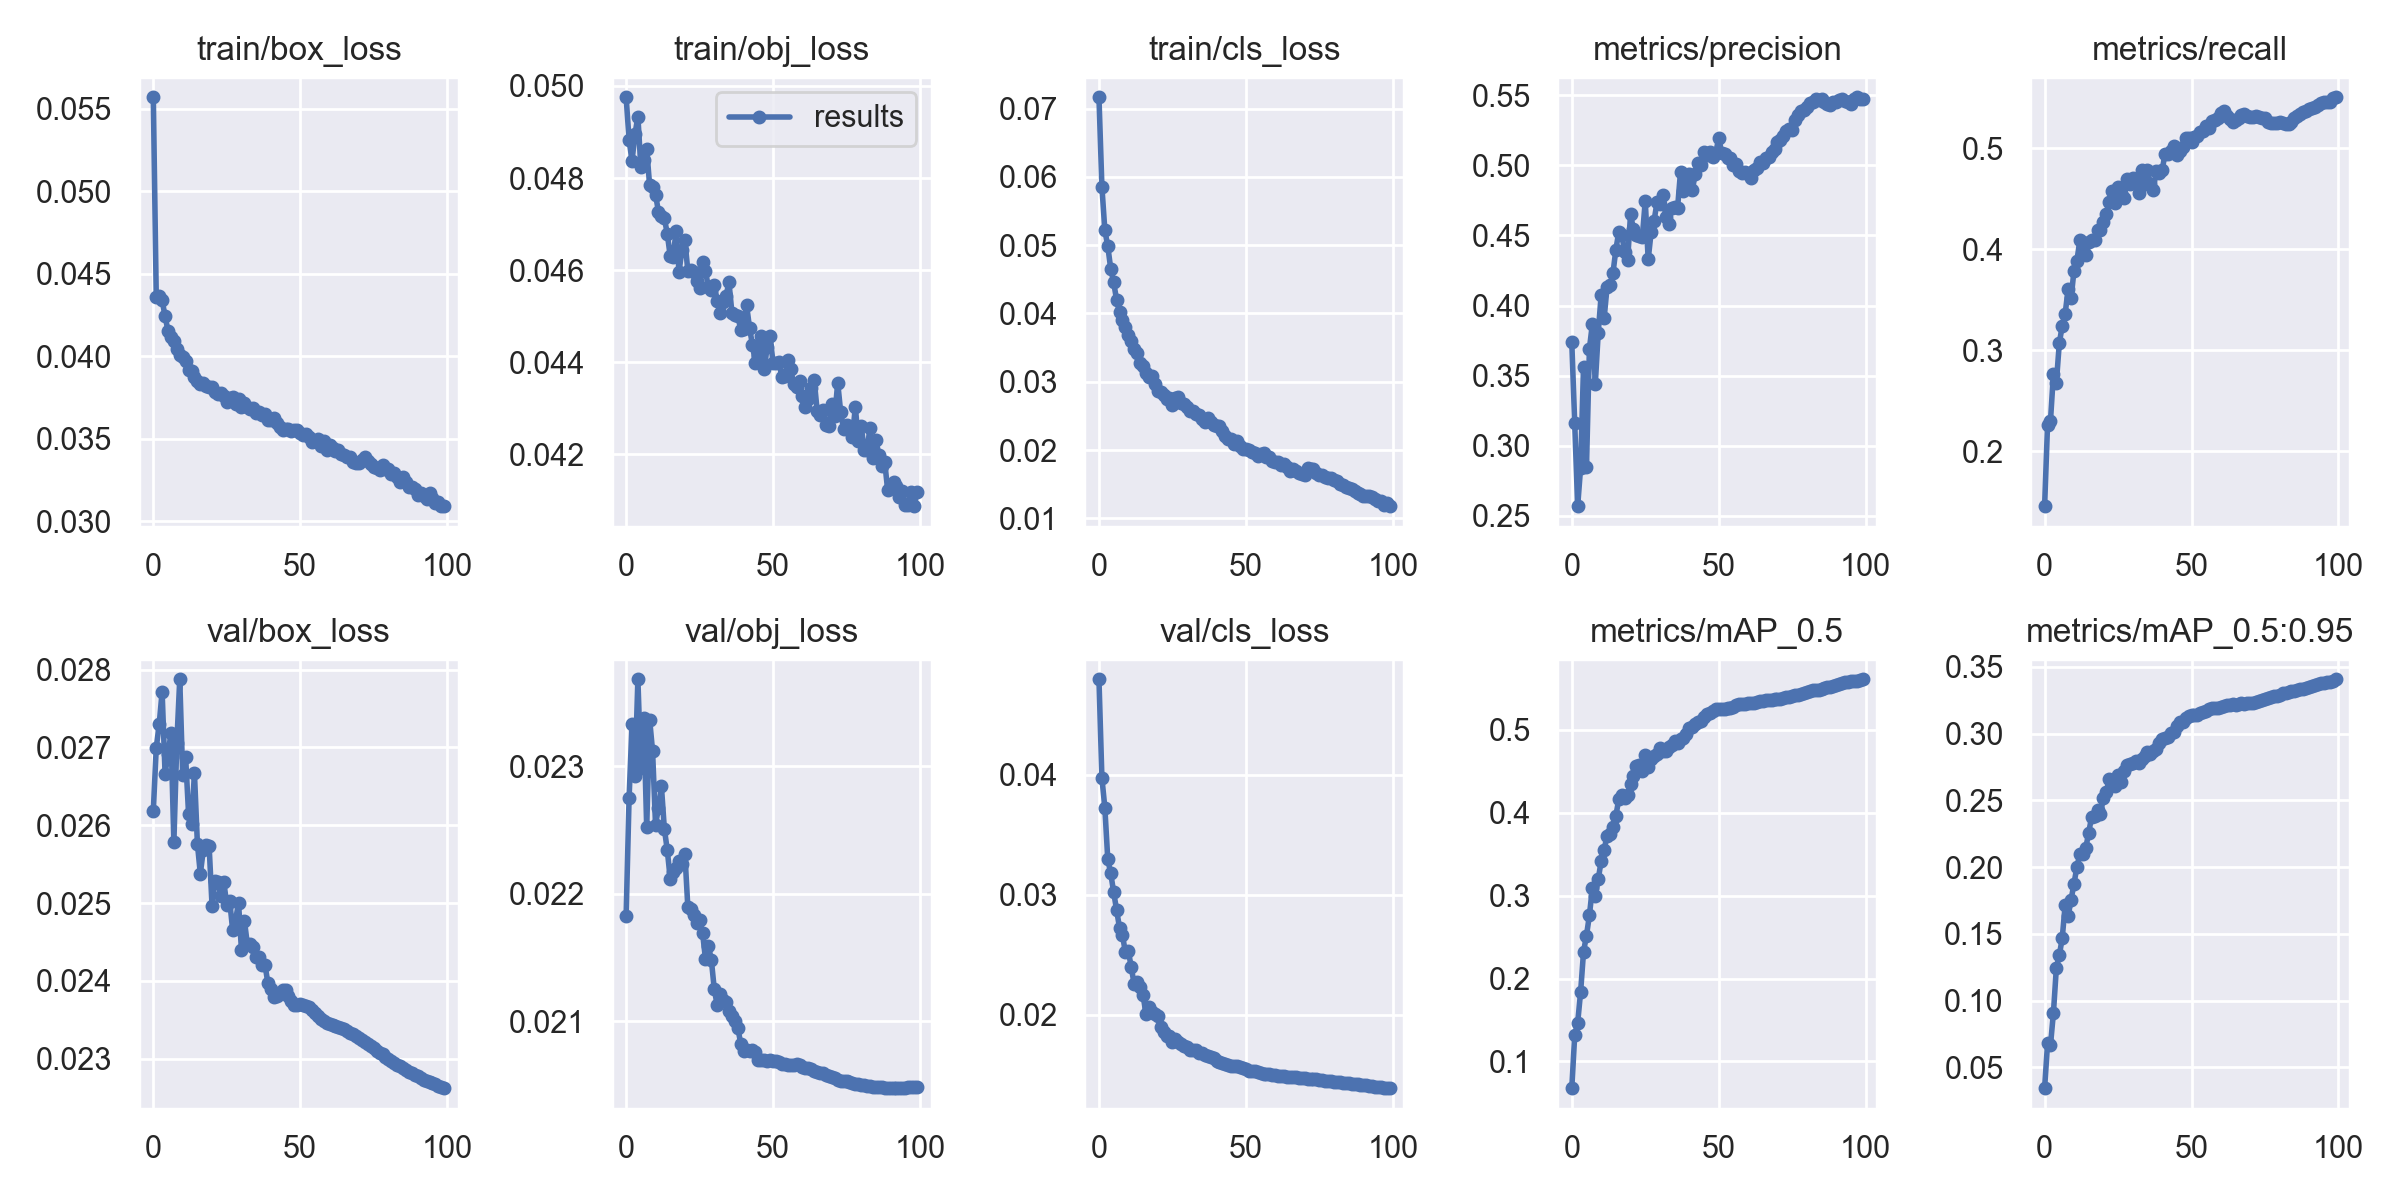
\includegraphics[width=0.92\textwidth]{results.png}
  \caption{训练与验证指标变化曲线}
\end{figure}

F1--Confidence 曲线显示，全类别综合 F1 的较优置信度阈值约为 0.135。实际系统默认阈值设置为 0.15，并允许用户调整。对于有害垃圾筛查，可以适当降低阈值以提高 Recall，但同时必须接受误报增加的代价。

\begin{figure}[H]
  \centering
  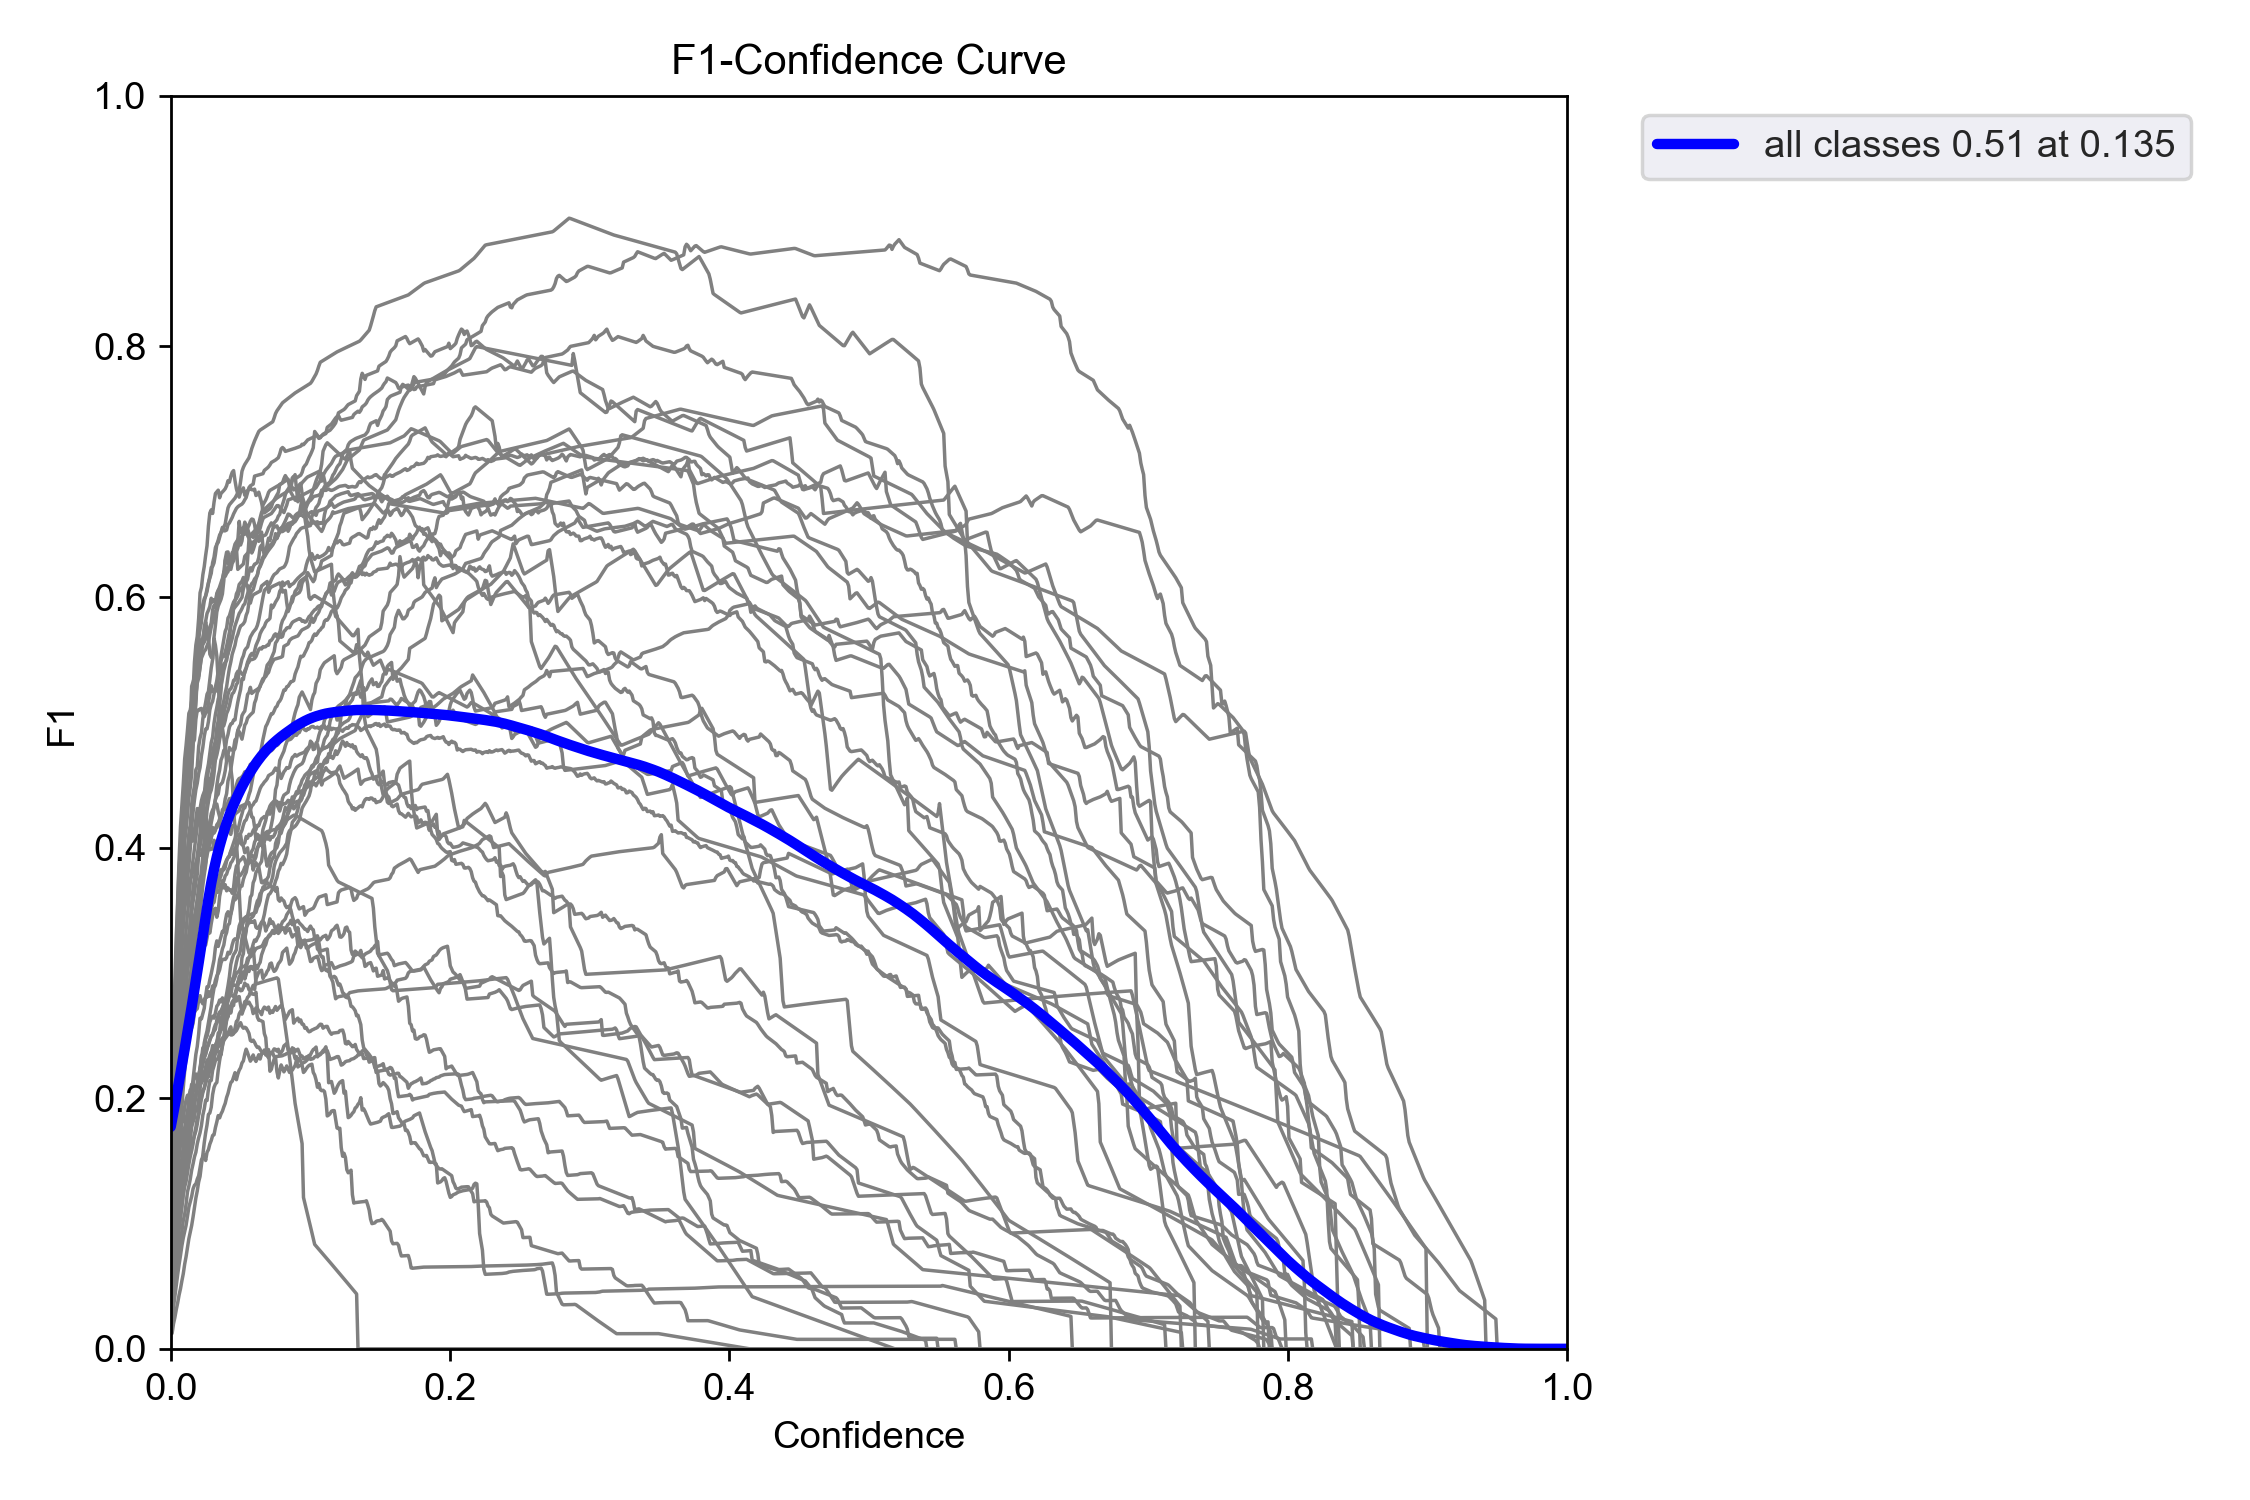
\includegraphics[width=0.78\textwidth]{F1_curve.png}
  \caption{F1 与置信度阈值关系}
\end{figure}

\subsection{验证集检测效果}

图~\ref{fig:val-comparison} 对比了验证集人工标注与模型预测结果。模型能够定位部分纸板、药膏、金属食品罐等目标，但仍存在漏检、类别混淆和低置信度问题。混淆矩阵也显示，不同类别的识别能力差异较大，且部分真实目标被判断为背景。

\begin{figure}[H]
  \centering
  \begin{subfigure}{0.48\textwidth}
    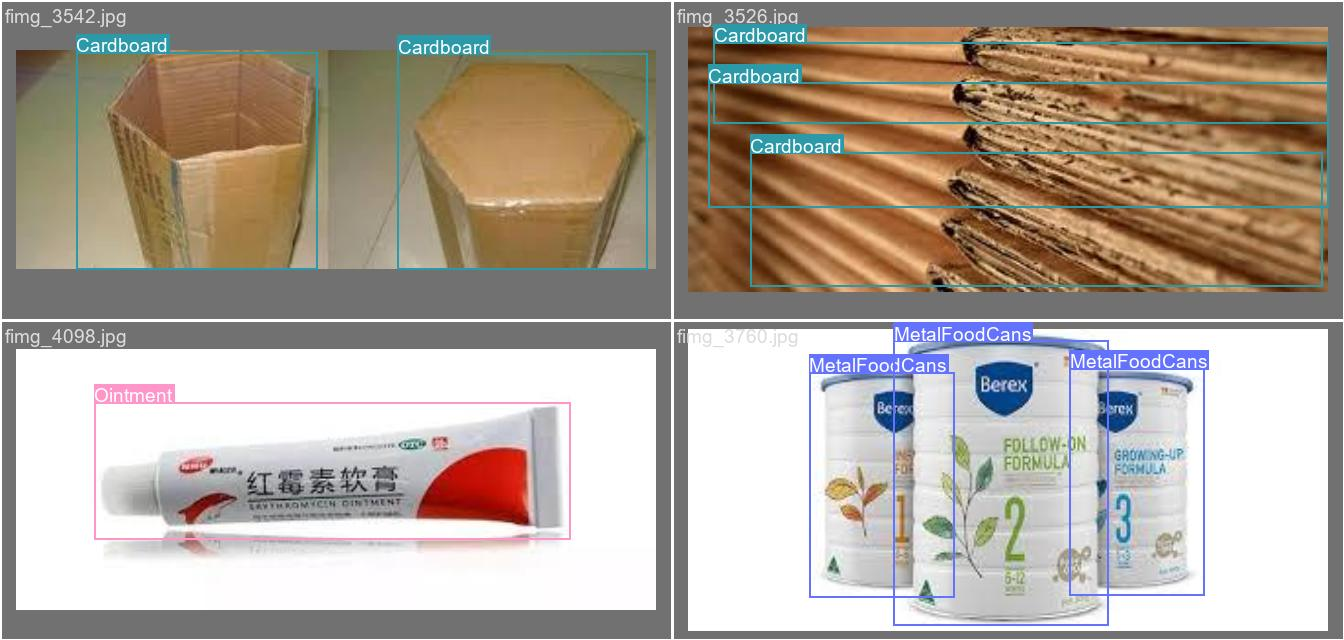
\includegraphics[width=\textwidth]{val_batch0_labels.jpg}
    \caption{验证集真实标注}
  \end{subfigure}
  \hfill
  \begin{subfigure}{0.48\textwidth}
    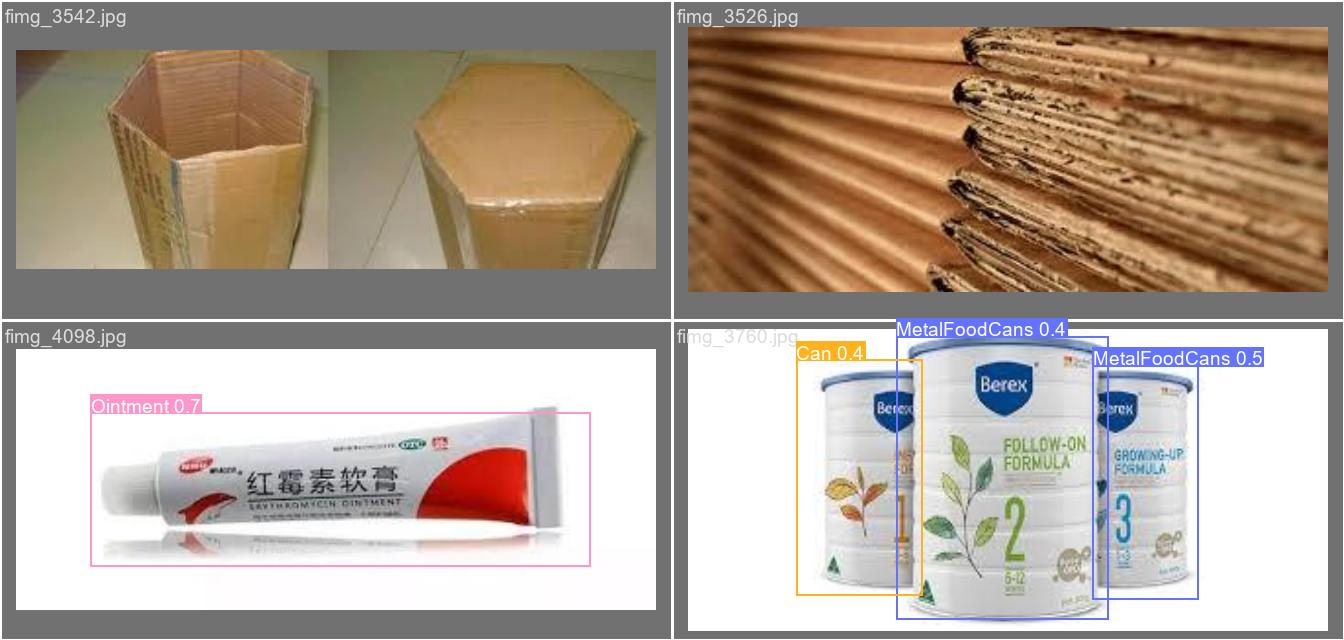
\includegraphics[width=\textwidth]{val_batch0_pred.jpg}
    \caption{模型预测结果}
  \end{subfigure}
  \caption{验证集标注与预测对比}
  \label{fig:val-comparison}
\end{figure}

\begin{figure}[H]
  \centering
  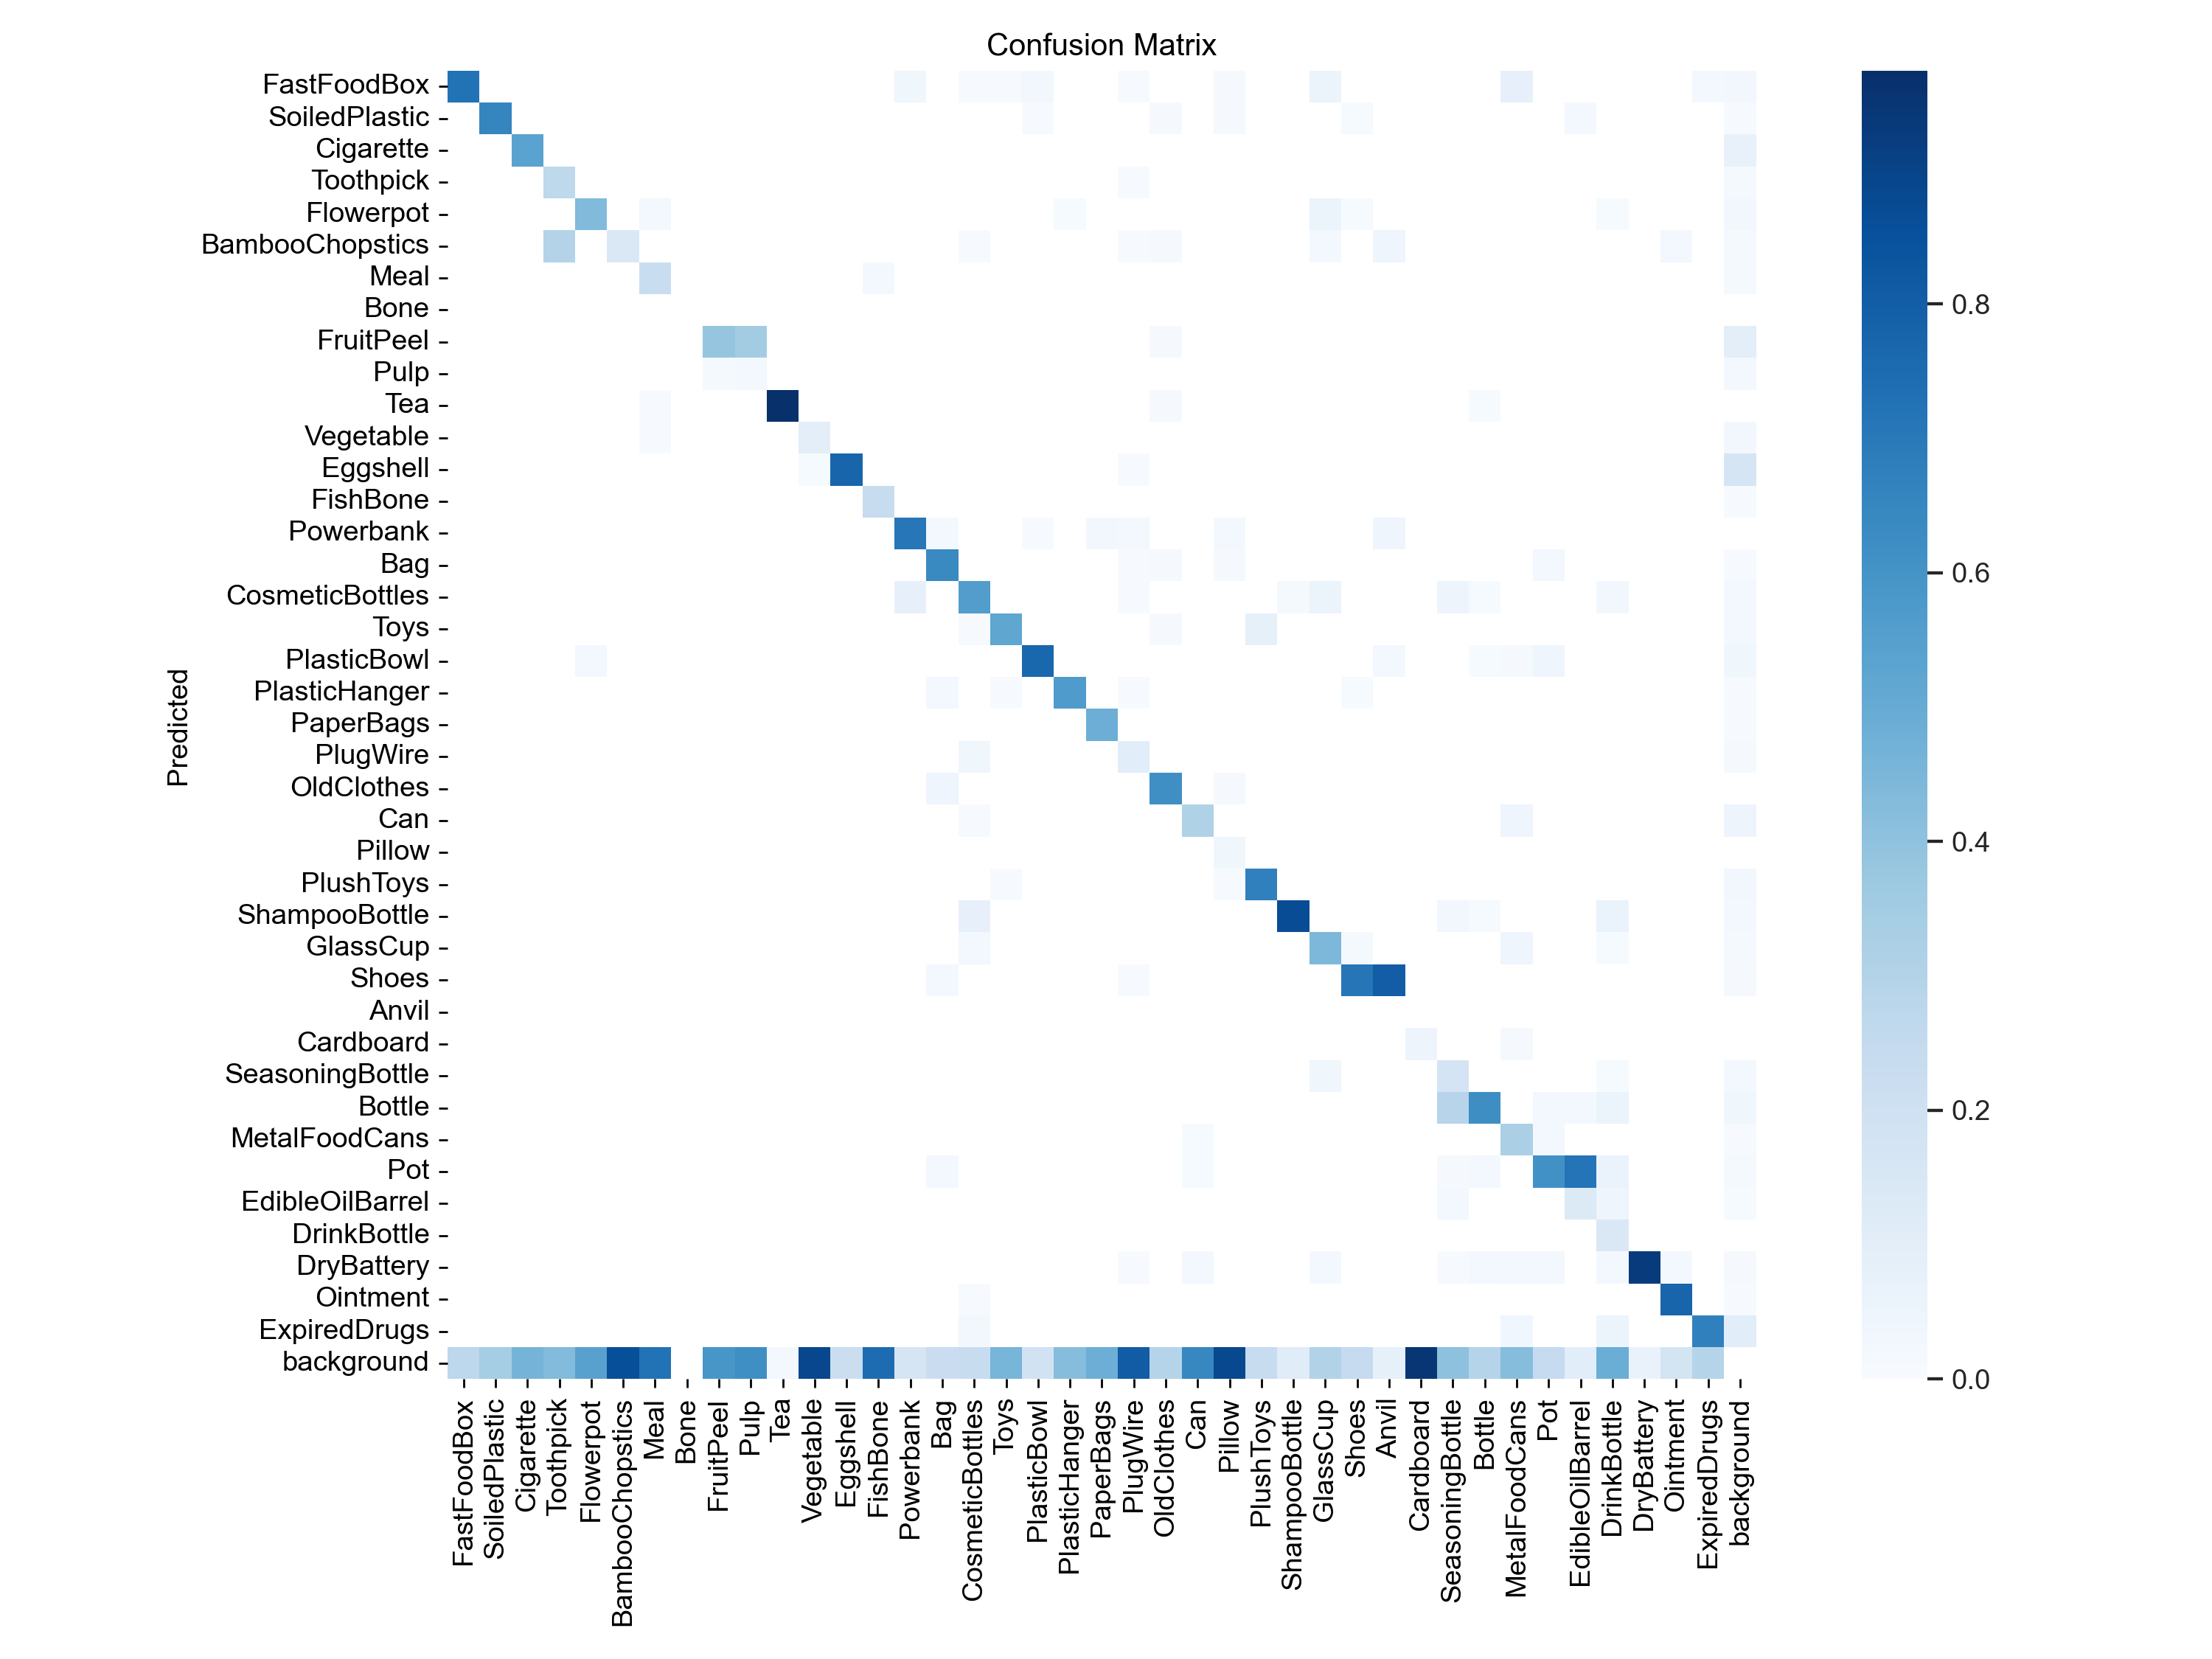
\includegraphics[width=0.92\textwidth]{confusion_matrix.png}
  \caption{模型归一化混淆矩阵}
\end{figure}

\subsection{有害垃圾检测与前端系统}

本项目将干电池、过期药品、药膏、充电宝和化妆品瓶配置为重点告警类别。服务端在启动时加载一次模型，用户上传图片后依次完成预处理、推理、类别统计和风险判断。若检测到有害垃圾，前端会使用红色提示区域展示有害类别及数量；若未检测到有害垃圾，则显示普通检测结果。前端还提供置信度阈值调整功能，便于在高召回和低误报之间进行权衡。

\begin{figure}[H]
  \centering
  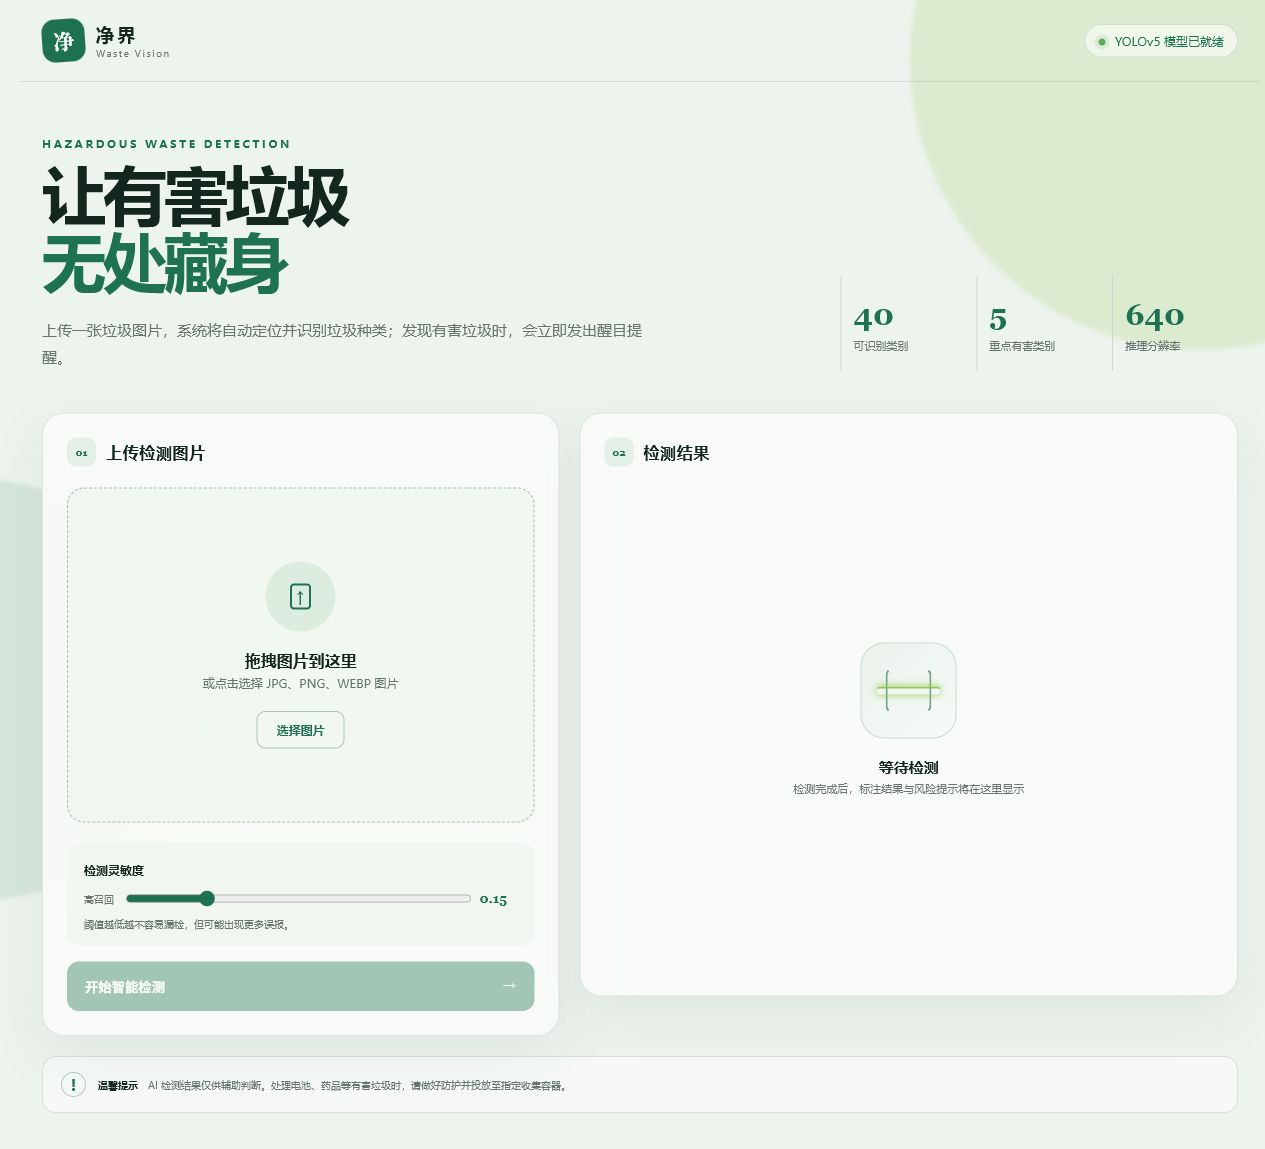
\includegraphics[width=\textwidth]{frontend.png}
  \caption{有害垃圾智能检测 Web 前端}
\end{figure}

Web 应用支持一键启动，完整 Pipeline 如下：

\begin{lstlisting}[caption={部署后的实际检测流程}]
Upload image
  -> EXIF orientation correction and RGB conversion
  -> preprocess.py
  -> YOLOv5 best.pt inference
  -> class counting and hazardous-waste decision
  -> annotated image and highlighted warning
\end{lstlisting}

\section{相关讨论}

\subsection{当前系统的有效性}

本项目的主要贡献是建立了一条完整、可运行的有害垃圾视觉筛查流程。相较于仅训练模型，本项目还将图像增强、有害类别判断、检测结果可视化和一键启动部署整合为可交互系统。该系统能够识别多类常见垃圾，并对部分常见有害垃圾进行重点提醒，从而初步验证了“拍摄垃圾堆图像并辅助环卫工人寻找有害垃圾”这一思路的可行性。

对于现实应用而言，本系统最有价值的输出并不是单纯给出垃圾名称，而是指出“哪里可能存在有害垃圾”。目标框能够帮助工作人员缩小检查范围，风险提示则能提醒工作人员采用更谨慎的处理方式。即使系统尚不能完全自动化分拣，它仍可作为人工操作前的辅助筛查环节。

\subsection{局限性分析}

\begin{enumerate}
  \item \textbf{训练域与真实垃圾堆存在差异。} 现有数据中包含较多背景干净、目标清晰的图片，而真实垃圾堆通常具有严重遮挡、污损和密集堆叠。
  \item \textbf{整体检测精度仍有限。} 当前 Precision 与 Recall 均约为 55\%，不能将模型输出视为最终判定结果。
  \item \textbf{类别粒度与有害属性并不完全一致。} 某些容器是否有害取决于其残留物，仅凭外观类别可能无法准确判断。
  \item \textbf{预处理并非在所有场景中都必然提升性能。} 增强对比度和锐化可能帮助观察暗部与边缘，也可能放大噪声。因此后续需要通过对照实验验证每个预处理组件对 mAP 和 Recall 的真实贡献。
  \item \textbf{当前缺少专门的垃圾堆独立测试集。} 若要证明系统能够稳定用于复杂垃圾堆场景，需要收集并单独标注真实混合垃圾图像进行测试。
\end{enumerate}

\subsection{YOLO26 与未来模型升级}

本实验使用 YOLOv5s 完成基线系统。经调研，Ultralytics 官方文档已发布 YOLO26，并将其描述为面向边缘设备的端到端视觉模型，强调免 NMS 推理和部署效率\cite{yolo26docs}。这些特性与本项目未来面向移动终端、现场设备和实时筛查的方向具有较高相关性。

不过，模型版本更新并不意味着在本项目数据集上必然获得更高效果。未来应在相同训练集、验证集、输入尺寸和评价指标下，对 YOLOv5s 与 YOLO26 的 Precision、Recall、mAP、推理速度和资源占用进行公平对照，再决定是否迁移。特别是本项目更关注有害垃圾漏检，因此模型升级评价应优先观察有害类别 Recall，而非只比较总体 mAP。

\section{总结与未来工作}

本项目针对环卫工人从大量混合垃圾中快速发现有害垃圾的现实需求，完成了从数据获取、图像预处理、YOLOv5s 迁移学习、检测效果分析到 Web 应用部署的完整实验。项目经历了自行拍摄和 AI 生成数据不足的问题，随后采用开源标注数据集扩大训练规模；同时结合 Resize、Gaussian Blur、CLAHE 和 Unsharp Masking 改善模型输入质量。最终系统能够输出垃圾类别和位置，并在检测到有害垃圾时进行重点提醒。

当前结果证明了方案的可行性，但距离实际稳定应用仍有差距。下一阶段计划包括：

\begin{enumerate}
  \item 收集真实垃圾堆、转运站和分拣现场图片，建立独立测试集；
  \item 增加干电池、药品、化学品容器等有害垃圾样本，尤其补充遮挡、污损、小目标和破损状态；
  \item 进行预处理消融实验，量化 Resize、去噪、CLAHE 和锐化的独立贡献；
  \item 针对有害垃圾类别调整损失权重与阈值，优先提升 Recall；
  \item 在同一数据集上比较 YOLOv5s 与 YOLO26 等模型的准确率、速度与部署成本；
  \item 将系统扩展到摄像头实时检测，并探索与自动分拣设备的联动。
\end{enumerate}

总体而言，本项目所解决的关键问题是：在有害垃圾进入下游处理环节之前，利用图像检测帮助工作人员更快地发现并分离风险目标。围绕这一目标继续优化数据、模型和部署方式，能够使系统逐步从课程实验原型发展为具有实际辅助价值的环境保护工具。

\section{团队成员贡献}

\begin{table}[H]
  \centering
  \caption{团队成员贡献说明}
  \begin{tabular}{p{3cm}p{10.5cm}}
    \toprule
    成员 & 主要贡献 \\
    \midrule
    刘晋嶂 & 负责 YOLOv5s 模型训练、训练参数设置、断点续训、权重选择及训练结果整理。\\
    邓荣基 & 负责图片处理方案设计与实现，包括 Resize、Gaussian Blur、CLAHE、Unsharp Masking 及预处理 Pipeline 接入。\\
    袁致朗 & 负责项目技术调研、现实应用价值分析、实验结果讨论与实验报告撰写。\\
    \bottomrule
  \end{tabular}
\end{table}

\appendix
\section{主要程序与使用方式}

\subsection{程序结构}

\begin{longtable}{p{5cm}p{9cm}}
  \toprule
  文件或目录 & 功能 \\
  \midrule
  \endhead
  \texttt{preprocess.py} & 图像尺寸调整、去噪、局部对比度增强与锐化。\\
  \texttt{train.py} & YOLOv5 模型训练与断点续训。\\
  \texttt{detect.py} & YOLOv5 基础图片检测程序。\\
  \texttt{exp12/weights/best.pt} & 验证集表现最好的模型权重。\\
  \path{hazardous_waste_web/app.py} & Web 服务、预处理 Pipeline、模型推理与有害垃圾判断。\\
  \path{hazardous_waste_web/static/} & 图片上传、结果展示和风险提示前端。\\
  \texttt{一键启动.bat} & 自动检查环境、加载模型并打开 Web 页面。\\
  \bottomrule
\end{longtable}

\subsection{运行方式}

\begin{lstlisting}[language=bash,caption={命令行启动方式}]
conda activate YOLO
python hazardous_waste_web/app.py
\end{lstlisting}

Windows 环境下也可以直接双击仓库根目录中的 \texttt{一键启动.bat}。项目代码仓库地址为：\url{https://github.com/AndyLongest/HarmfulGarbageDetector.git}。

\begin{thebibliography}{9}
  \bibitem{yolov5repo}
  Ultralytics.
  \newblock YOLOv5 GitHub Repository.
  \newblock \url{https://github.com/ultralytics/yolov5}.

  \bibitem{yolo26docs}
  Ultralytics.
  \newblock YOLO26 Documentation.
  \newblock \url{https://docs.ultralytics.com/models/yolo26/}.

  \bibitem{clahe}
  Karel Zuiderveld.
  \newblock Contrast Limited Adaptive Histogram Equalization.
  \newblock In \emph{Graphics Gems IV}, 1994.
\end{thebibliography}

\end{document}
